%Papierformat, mit Koma-Script Dokumentenklasse (Europäisches Design)
\documentclass[12pt,a4paper]{scrartcl}
%Deutsche Silbentrennung
\usepackage[ngerman]{babel}
%Listen einrücken
\usepackage{enumitem}
%Deutsche Umlaute
\usepackage[utf8]{inputenc}
%Trennung von deutschen Umlauten
\usepackage[T1]{fontenc}
%Bibtex für Zitate,
% see: https://en.wikibooks.org/wiki/LaTeX/Bibliography_Management#Customization
\usepackage[]{natbib}
%Grafikpaket laden
\usepackage{graphicx}
%Grafik Floating einschränken
\usepackage{placeins}
%Referenzierung mit Name
\usepackage{titleref}
%Unterschritszeilen
\usepackage{tabularx}
%Verlinkung
% see:https://en.wikibooks.org/wiki/LaTeX/Hyperlinks
\usepackage[hidelinks]{hyperref}
%Urls sollen erkannt werden
\usepackage{url}
%Ermöglicht es von Schrift umflossene Bilder und Tabellen einzufügen
\usepackage{wrapfig}
%Sourcecode anzeigen lassen
\usepackage{listings}
%Farbenpaket laden
\usepackage{xcolor}
%Einrichten des Linking
%\hypersetup{
%    colorlinks,
%    linkcolor={red!50!black},
%    citecolor={blue!50!black},
%    urlcolor={blue!80!black}
%}
%Umbennen der Bibliography Angabe in Literatur
\renewcommand{\bibname}{Literatur}
%Festlegung des Zitierstiles
\bibliographystyle{plain}
%Inhaltsverzeichnis Tiefe erweitern
\setcounter{tocdepth}{5}
%Nummerierung Tiefe erweitern
\setcounter{secnumdepth}{5}

%\makeatletter
%\newcommand\footnoteref[1]{\protected@xdef\@thefnmark{\ref{#1}}\@footnotemark}
%\makeatother​

%Dokumentbeginn
\begin{document}
	
	\begin{titlepage}
	%Eine mbox wird verwendet um Text zusammenzuhalten
	%vspace erzeugte die in Klammern angegebenen Zeilenabstände
	%baselineskip setzt zeilenabstand
   	\mbox{}\vspace{5\baselineskip}\\
   	%Schriftart und Größe als Attribut
   	\rmfamily\huge
   	%Mittige Textausrichtung (\centerline für eine Zeile)
   	\centering
   	%Das Argument erscheint in Kapitaelchen (small capitals).
	\textsc{Weiterentwicklung von Hablame}
	%Umbruch bezogen auf die Hoehe des Kleinbuchstaben x in diesem Element * Faktor
	\\[3ex]
   	Projektarbeit
   	\rmfamily\Large
   	\vspace{1\baselineskip}\\
   	%Externes einbinden einer Textdatei
   	%% versionsnummer entfernt
   	%\input{version.txt}\mbox{}
	\vspace{3\baselineskip}
	Hochschule für angewandte Wissenschaften Würzburg-Schweinfurt
   	\vspace{5\baselineskip}\\
   	\rmfamily\Large
   	David Artmann\\
   	\rmfamily\Large
   	Dominik Hirsch\\
   	\rmfamily\Large
   	Kristoffer Schneider
   	\vspace{1\baselineskip}\\
   	%Heutiges Datum
   	\today
\end{titlepage}

	%Inhaltsverzeichnis
	\tableofcontents
	\newpage
	
	%Abbildungsverzeichnis
	\listoffigures
	

	%\newpage
	%\bibliography{general/bibtex/bibtex.bib}
	%Bibliography im Inhaltsverzeichnis anzeigen(muss unterhalb von bibliography
	% sein)
	\addcontentsline{toc}{section}{Literatur}
	\newpage
	
	\section{Allgemeine Änderungen}

\subsection{Organisatorisches}
\subsubsection{Struktur der Repositories}
Das ursprüngliche Projekt bestand aus zwei Teilen: der Android App, als
Client, und einem Java Backend, welches den Bot beinhaltete und die Server
Rolle einnahm. Das Versionsmanagement beider wurde bisher in einem gemeinsamen
Repository gehandhabt. Dies brachte eine gewisse Unübersichtlichkeit
mit sich. Daher haben wir für jedes Teilprojekt ein eigenes Repository angelegt.
Die Aufteilung zwischen der App und dem Backend wurde beibehalten, es kam
lediglich noch ein Teil hinzu, welchen die Service-API-Library ausfüllt. Damit
ist die aktuelle Aufteilung auf Github wie folgt:\\\\
\begin{small}
\begin{tabular}{ l l }
Altes Repository unserer Vorgänger: & https://github.com/TeamChatbot/chatbot\\
Aktuelle Android App: & https://github.com/TeamChatbot/Hablame-Android-App\\
Aktuelle Service-API-Library: &
https://github.com/TeamChatbot/hablame-service-api\\
Aktuelles Service-Botbackend: &
https://github.com/TeamChatbot/Hablame-BotBackend\\
\end{tabular}
\end{small}\\\\
Durch diese Aufteilung kann besser und unabhängiger an den einzelnen Teilprojekten gearbeitet werden.

\subsubsection{Aktuelle Aufgabenverteilung auf die Teilprojekte}
Durch das Hinzufügen der Service-API-Library ergibt sich nachfolgend dargestellter Gesamtaufbau.\\
\begin{figure}[h]
	\centering
	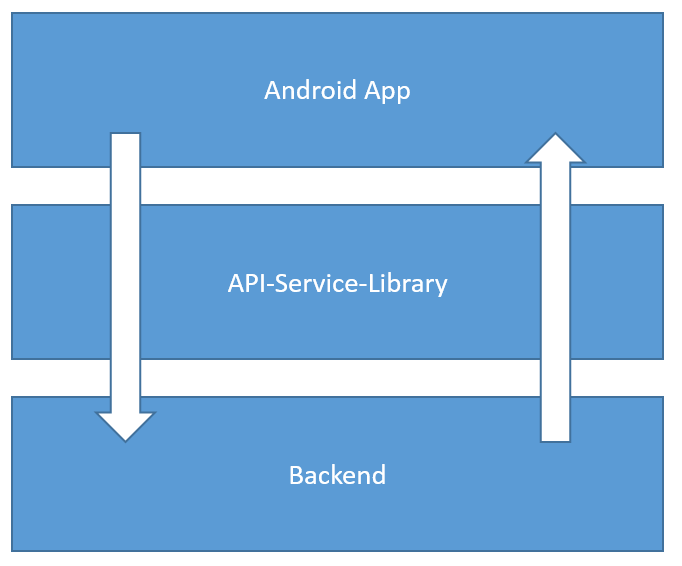
\includegraphics[width=0.7\linewidth]{ks/graphics/arch.png}
	\caption{Gesamtaufbau Hablame}
	\label{fig:arch}
\end{figure}\\
Jedes Teilprojekt behandelt ein Teilproblem des Gesamtsystems.\\
Android App:
\begin{itemize}\itemsep0pt
	\item Umwandlung gesprochener Sprache in Text ("Speech-To-Text")
	\item Umwandlung von Text in gesprochene Sprache ("Text-To-Speech")
	\item Weiterleiten der Informationen mittels der API-Service-Library an das Backend
\end{itemize}
API-Service-Library:
\begin{itemize}\itemsep0pt
	\item Erstellen der Anfragen an das Backend
	\item Weitergabe der Backend-Antworten an das aufrufende System
\end{itemize}
Backend:
\begin{itemize}\itemsep0pt
	\item Hosting und Konfiguration des Chatbots
	\item Auswerten der Serviceanfragen
\end{itemize}

\subsection{Dokumentation im Allgemeinen}
Für die Dokumentation gibt es nun mehrere Anlaufstellen. In Redmine gibt es ein
integriertes Wiki welches wir bereits mit einigen Informationen zu allgemeine
Dingen wie Logindaten und den einzelnen Repositories, aber auch zu genutzten
Technologien wie beispielsweise das Git-System gefüllt.\footnote{Projekt Wiki
in Redmine: http://194.95.221.229/redmine/projects/hablame/wiki/} Zusätzlich zu
dem Wiki gibt es in jedem Repository ein Readme, das nochmal zusätzlich einen
Überblick über das dortige Projekt gibt.\\
Die Dokumentation des Programmcodes ist mittels dem Java Tool JavaDocs
umgesetzt worden. Die damit generierten Dokumentationsseiten sind im jeweiligen
Repository auf Github zu finden.

\subsection{Unit Testing}
Neu ist auch das, bisher nicht beachtete, automatisierte Testen des
Programmcodes. Hierfür wird auf das Java Framework JUnit
zurückgegriffen.\footnote{Projektseite von JUnit: http://junit.org/} Durch das
Nutzen eines solchen Frameworks ist es möglich automatisiert Programmcode auf
die korrekte Ausführung zu testen. Gerade in einem großen System wie das
Backend nimmt das einiges an arbeit ab, während es die Wartbarkeit deutlich erhöht.\\
Aktuell wird es sowohl im Backend, als auch in der Service-API-Library genutzt.\\
Im Backend werden zusätzlich noch die Mockito Bibliotheken genutzt, da es mit
diesen ermöglicht wird zusätzlich noch die Controller-API zu testen, welche den
Chatbot von außen über Requests erreichbar und ansprechbar macht.

\subsection{Build Management mit Maven}
Ein Problem im bisherigen Projekt war, dass Abhängigkeiten und der Buildvorgang
nicht zentral geregelt wurden. So wurden genutzte Bibliotheken als Jar-Archive
eingebunden. Dies hat zur Folge das diese Bibliotheken zu meist händisch in das
Arbeitssystem geladen werden müssen. Um dies zu vereinfachen und den
Buildvorgang zu vereinheitlichen wird im Backend sowie der Service-API-Library
nun das Build Management Tool Maven verwendet.\footnote{Projektseite von Maven:
https://maven.apache.org/} Somit gibt es jetzt in beiden Projekten einen
einheitlichen Punkt für die Konfiguration der Abhängigkeiten und des
Buildvorgangs, die pom.xml.


	\newpage
	
	\section{Die Service-API-Library}
Um die Nutzung des Backends zu vereinfachen wurde ein weiteres Teilprojekt erstellt: die Service-API-Library. Dieses Projekt bietet einen einfach zu handhabenden Client zur Nutzung des Bot-Services. Dafür bietet dieser Methoden zur jeder Schnittstelle des Backends.\\
Durch dieses Vorgehen ergibt sich der Vorteil, dass somit eine einheitliche, leicht zu nutzende Schnittstelle für Nutzerprogramme geboten wird, welche auch in weiteren Anwendungen integriert werden kann (z.B. in eine Desktopanwendung).\\
Als Basis für die Rest-Kommunikation wird die Bibliothek UniREST von Mashape verwendet.\footnote{Unirest: http://unirest.io/}\\
	\newpage
	
	\section{Überarbeitung der Server-Architektur}
	Im Rahmen der Projektarbeit soll die serverseitige Architektur überarbeitet
	und mit der Nutzung von modernen Tools und Frameworks ausgestattet werden.
	Diese Optimierungen werden in den folgenden Unterkapiteln beschrieben.
	
	\subsection{Datenbank}
		Eine Anforderung an das Projekt war es, dass die bisherige Nutzung einer
		Oracle Datenbank abgelöst wird durch eine frei verfügbare Datenbank. Das Team
		entschied sich für das freie relationale Datenbankmanagementsystem MySQL in
		der aktuellsten produktiven Version 5.6.26 zum Zeitpunkt dieser Arbeit.
		Dies bringt den großen Vorteil mit sich, eine weitverbreitete quelloffene, statt
		einer proprietären Datenbank Software zu nutzen.
		
	\subsection{Das Spring Framework}
		Eine weitere Anforderung stellt die Nutzung moderner Frameworks und
		Technologien dar. Um einerseits einen guten Programmierstil sicher stellen zu
		können und andererseits die Kollaboration zu verbessern, sowie zukünftigen
		Projektteams den Einstieg maßgeblich zu erleichtern.
		Spring ermöglicht es durch so genannte Annotationen die Persistierung von
		Objekten unter Zuhilfenahme von Hibernate mit Object-Relational-Mapping zu
		vereinfachen. Zusätzlich wird das Testen mit Unittests durch JUnit
		simplifiziert und die Instanziierung von Objekten zur Laufzeit im
		Singleton-Pattern durchgeführt. Das Speichern und Lesen von Objekten kann
		unter Spring beispielsweise durch Interfaces mit der @Respository Annotation
		übernommen werden. So ist es möglich ohne eine SQL Anweisung selbst zu
		schreiben, Datenbankzugriffe zu realisieren und mit Objekten zu arbeiten.
		Dies erleichtert das Erstellen der Daten-Zugriffsschicht enorm. Diese
		Fähigkeit wird durch das Beerben des Interfaces CrudRepository, oder eines
		davon erbenden Interfaces erworben. Das Beerben eines dieser Interfaces
		verpflichtet zu den grundlegenden Datenbankoperationen Create, Read, Update
		und Delete eines spezifischen Objekttyps. Somit können POJOs in der
		Datenbank direkt abgespeichert werden. Diese werden in Form von separaten
		Model-Klassen angelegt, mit der @Entity Annotation versehen und sind somit
		als Datenbank-Entität gekennzeichnet. Weiterhin kann der Tabellenname, sowie
		einzelne Spaltennamen angegeben werden und Kardinalitäten zu anderen POJOs
		festgelegt werden, z.B. hat eine Kategorie mehrere Themengebiete.\\
		Die Spring Hierarchie ist ein wesentlicher Bestandteil der neu designten
		Server-Architektur und soll hier deshalb zusätzlich Einzug erhalten. Wie
		bereits erwähnt können einzelne Interfaces mit der @Repository Annotation für
		ORM genutzt werden. Diese Datenbankschicht der Hierarchie ist die unterste
		der drei und wird von der darüber befindlichen Service-Ebene genutzt. Hier
		werden Klassen mit der @Service Annotation zum Service ermächtigt, was dem
		Spring Kontext mitteilt, dass diese Services zur Laufzeit als Singleton
		Instanziiert werden. Services nutzen also die darunter liegenden Repositories
		für den Datenbankzugriff und verarbeiten die Daten weiter, bzw. führen andere
		gewünschte Operationen aus. Services stellen also Logikschicht dar. Diese
		Logikschicht wird von der API, den sogenannten Controllern genutzt, um
		Anfragen, sogenannte Web-Requests in Form eines GET oder POST, weiter
		bearbeiten zu können. Ein Controller hält die @Autowired Annotierten Services
		und dieser wiederum die Repositories und diese Objekte werden zur Laufzeit
		Instanziiert.
	\newpage
	
	\section{Überarbeitung der Android Application}

	\subsection{Motivation und Ziel}\label{motiv}
	Da die bisher vorhandene native Android Anwendung mit dem Hauptaugenmerk auf das Prototyping entwickelt wurde und aus diesem Grund kein spezielles Design sein eigen nennen kann, haben wir uns dazu entschieden, die Application von ihrem Status als Prototyp weg weiter zu entwickeln.\\
	Das Hauptaugenmerk sollte auf einer einfachen und verständlichen Bedienung sowie der Erstellung eines individuellen Designs liegen. Bestand die vorhandene App bisher nur aus einer Activity in welcher alle Interaktionen mit dem System ausgeführt wurden, so wurde die neue Anwendung etwas entzerrt und auf zwei Activities aufgeteilt. Auf diese beiden wurde die Nutzerführung und das gesamte Bedienkonzept angepasst und überarbeitet.\\

	\begin{figure}[htbp]
		\centering
		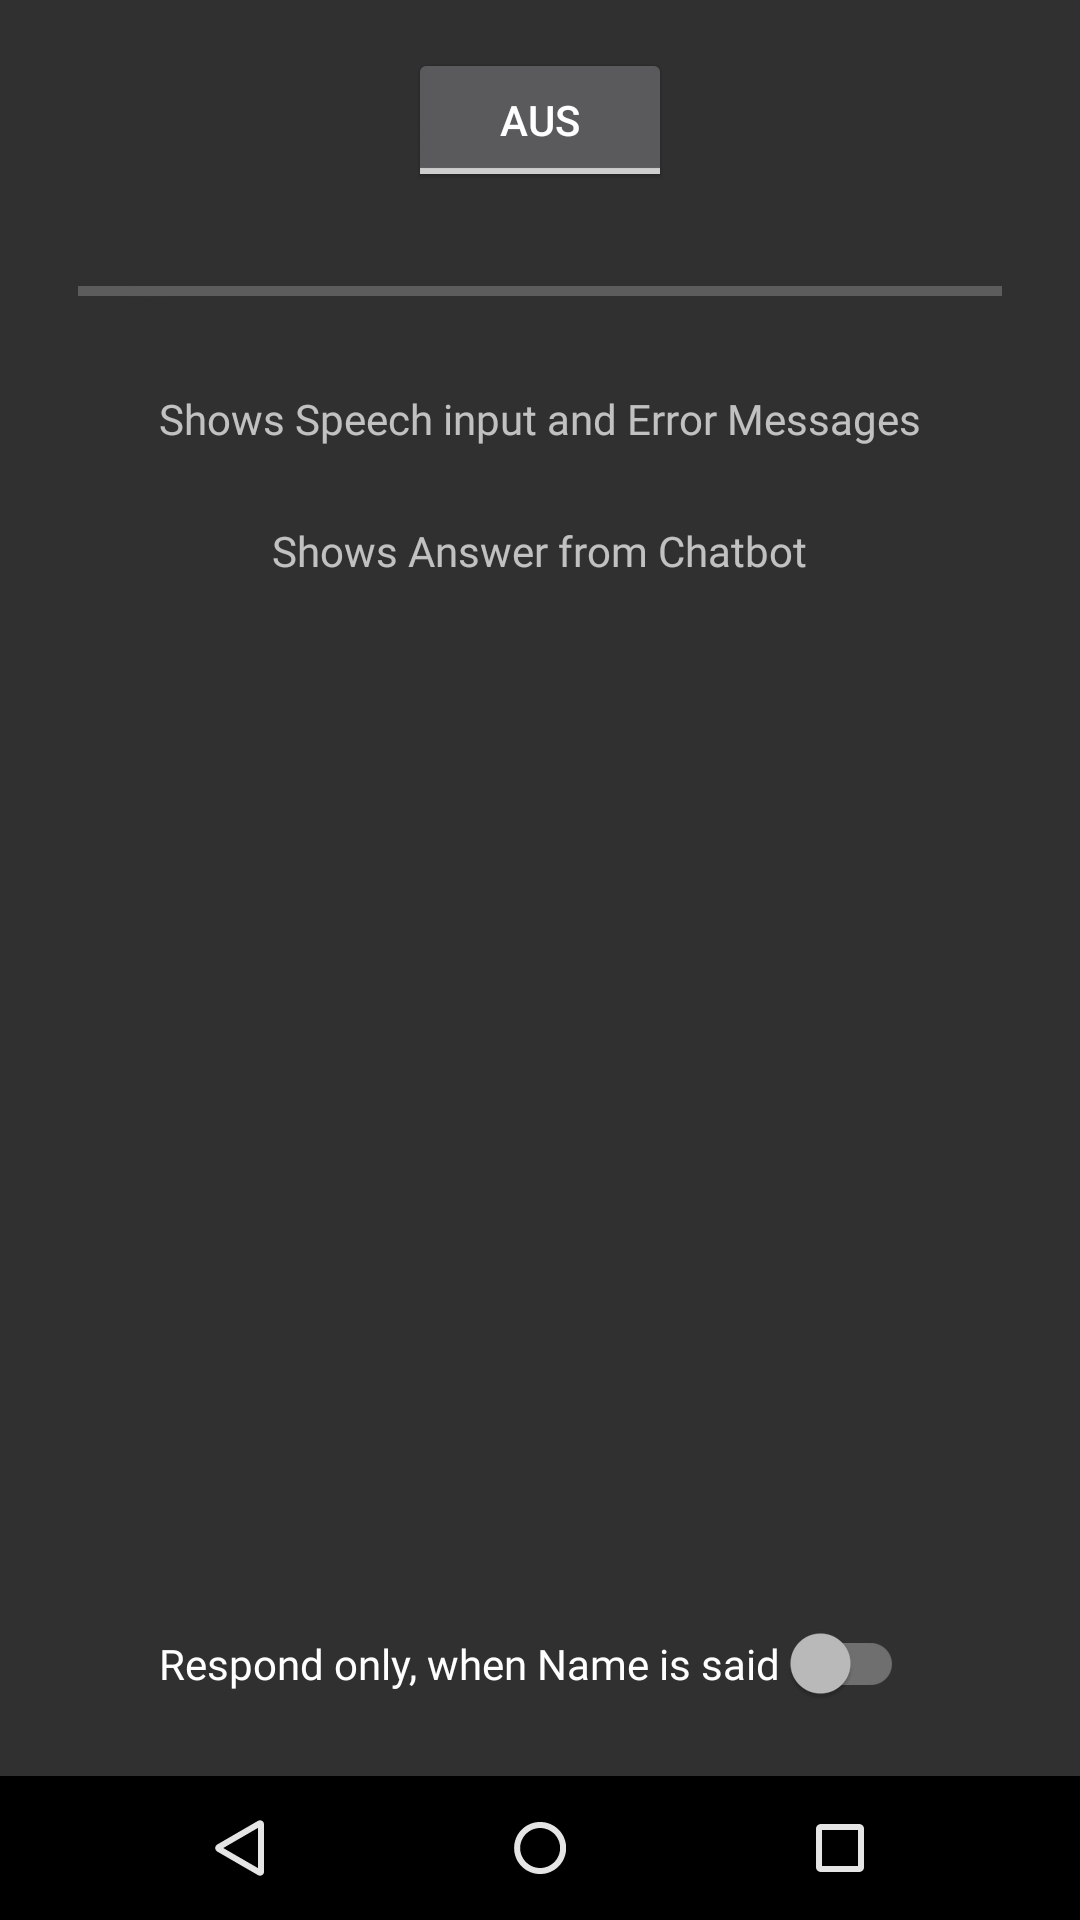
\includegraphics[height=0.8\textwidth]{dh/graphics/hablame-old.png}
		\caption{UI der bisherigen Android App}
		\label{fig:hablame-old}
	\end{figure} \leavevmode \\

	\subsection{Aufbau}\label{aufbau}

	Wie unter \ref{motiv} "Motivation und Ziel"' auf S.\pageref{motiv} bereits erwähnt, sollte die Anwendung auf zwei Activities aufgeteilt werden. Desweiteren beinhaltet sie eine Klasse für den zur Spracherkennung notwendigen Service - "RecognitionService.java" - und eine Klasse in welcher die möglichen Fehler des Service beschrieben werden, ErrorDescription.java. \\
	
	Bestandteile:
	\begin{itemize}\itemsep0pt
		\item MainActivity.java
		\item ConversationActivity.java
		\item RecognitionService.java
		\item ErrorDescription.java
	\end{itemize}
	
		\subsubsection{MainActivity}\label{mainact}
		Die MainActivity wird bei Programmstart automatisch geöffnet und bildet somit die Landing-Page. Sie besteht aus 3 grundlegenden Bereichen, nämlich dem Header, dem Body und dem Footer. Im Header sind die Schriftzüge "Háblame"' sowie "Das sprechende Faultier"' zu lesen.\\
		Der Body beinhaltet zum einen das Logo und ein editierbares Textfeld welches Nutzereingaben entgegennimmt, in diesem Fall speziell den Nutzernamen. Der Body bietet somit im Gegensatz zum Header eine Interaktionsmöglichkeit für den Nutzer.\\
		Der Footer besteht einzig aus einem Button welcher die komplette Displaybreite nutzt und bei einer onClick-Aktion auf die ConversationActivity weiterleitet. Diese Weiterleitung jedoch funktioniert nur wenn durch den Benutzer ein Username vergeben wurde, ansonsten wird eine Meldung auf dem Bildschirm ausgegeben, das kein Benutzername eingetragen ist. \\

		\subsubsection{ConversationActivity}\label{convact}
		
		Die ConversationActivity wird durch einen Intent in der MainActivity aufgerufen. Sie besteht ebenfalls aus Header Body und Footer. Änderungen gegenüber der MainActivity sind die Konversationsansicht im Body sowie eine andere Funktion des Buttons im Footer. Dieser bringt den Nutzer zurück in die MainActivity.\\
		Nach aufrufen der ConversationActivity wird der RecognitionService gestartet und der in der MainActivity zuvor eingegebene Nutzername in die Konversationsansicht übernommen.\\
				
		\subsubsection{RecognitionService und ErrorDescription}\label{recogError}
		Der RecognitionService welcher zur Erkennung der Sprache des Nutzers und deren Umsetzung in Text dient - und vice versa, wurde rein funktionell fast im Original übernommen. Einzig die Einbindung des alten Webservice wurde durch die Entwicklung und den Einsatz der Service-API-Library obsolet.\\
		Die Klasse ErrorDescription dient lediglich dem RecognitionService dazu um im Fehlerfall eine detaillierte Fehlerbeschreibung an den Nutzer zurück zu liefern.

	\subsection{Funktionsweise}\label{funktion}
	
	\begin{figure}[htbp]
		\centering
		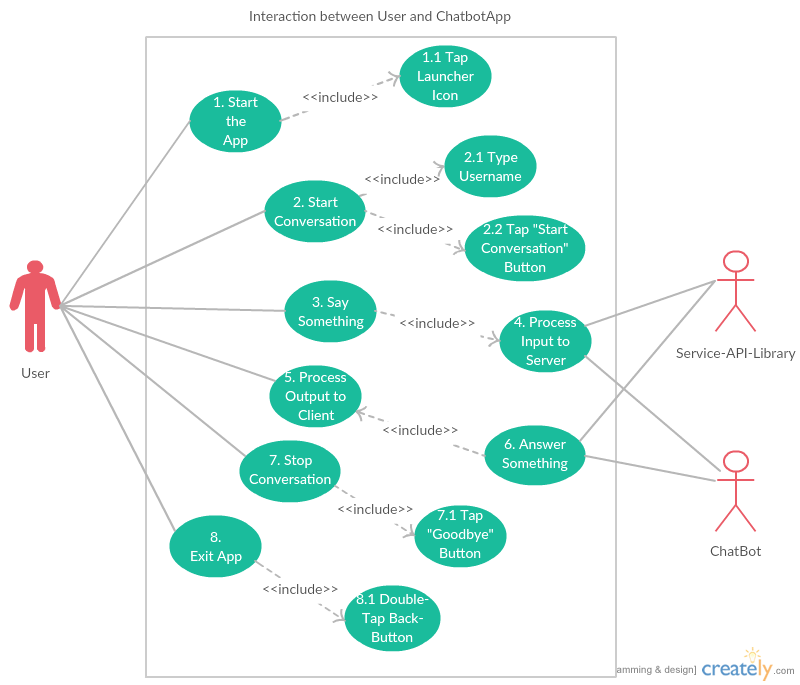
\includegraphics[height=0.9\textwidth]{dh/graphics/UseCaseChatbotApp.png}
		\caption{Use Case Diagramm zur Nutzung der App}
		\label{fig:usecaseapp}
	\end{figure} \leavevmode \\
	
	\subsection{Designanmerkungen}\label{design}
	
	Kritikpunkte bei der Erstellung:
	\begin{itemize}\itemsep0pt
	\item Entzerrung der Nutzerführung
	\item Erstellung eines Logos
	\item Wiedererkennungswert schaffen
	\item Individualität\\
	\end{itemize}
	Das UI wurde so erstellt um eine möglichst hohe Darstellbarkeit zu gewährleisten und der Fragmentierung auf Android bei zu kommen. So wurden bis auf das Logo selbst alle Elemente mit Android eigenen Bordmitteln umgesetzt um responsive zu bleiben. Das Logo wurde aus selbigem Grund in allen Auflösungen von ldpi bis xxhdpi umgesetzt.\\
	Eingesetzt wurde die, für kommerzielle sowie private Zwecke, frei nutzbare Schriftart Logobloqo2.ttf von seextwood\footnote{\label{foot:1}http://www.dafont.com/de/logobloqo2.font}. Sowie die Grafik "Cartellone con bradipo"' von bradisoft\footnote{\label{foot:2}https://de.fotolia.com/id/60029011}, die auf http://www.fotolia.de erworbene Vektorgrafik ist lizenzfrei und zeitlich sowie räumlich ohne Beschränkung nutzbar.\\
	
	\subsubsection{Farben}\label{farben}
		
		Alle verwendeten Farben sind dem Google Design Guide entnommen\footnote{\label{foot:3}https://www.google.com/design/spec/style/color.html\#color-color-palette}.\\
		
	MainActivity:
		\begin{itemize}\itemsep0pt
			\item Red 500
			\item Red 50
			\item Grey 400
		\end{itemize}
	
	ConversationActivity:
		\begin{itemize}\itemsep0pt
			\item Green 500
			\item Red 50
			\item Grey 400\\
		\end{itemize}
	Um die gestartete Konversation zu verdeutlichen, wurde für die ConversationActivity bewusst eine andere Hauptfarbe gewählt.
	
	\begin{figure}[htbp]
		\centering
		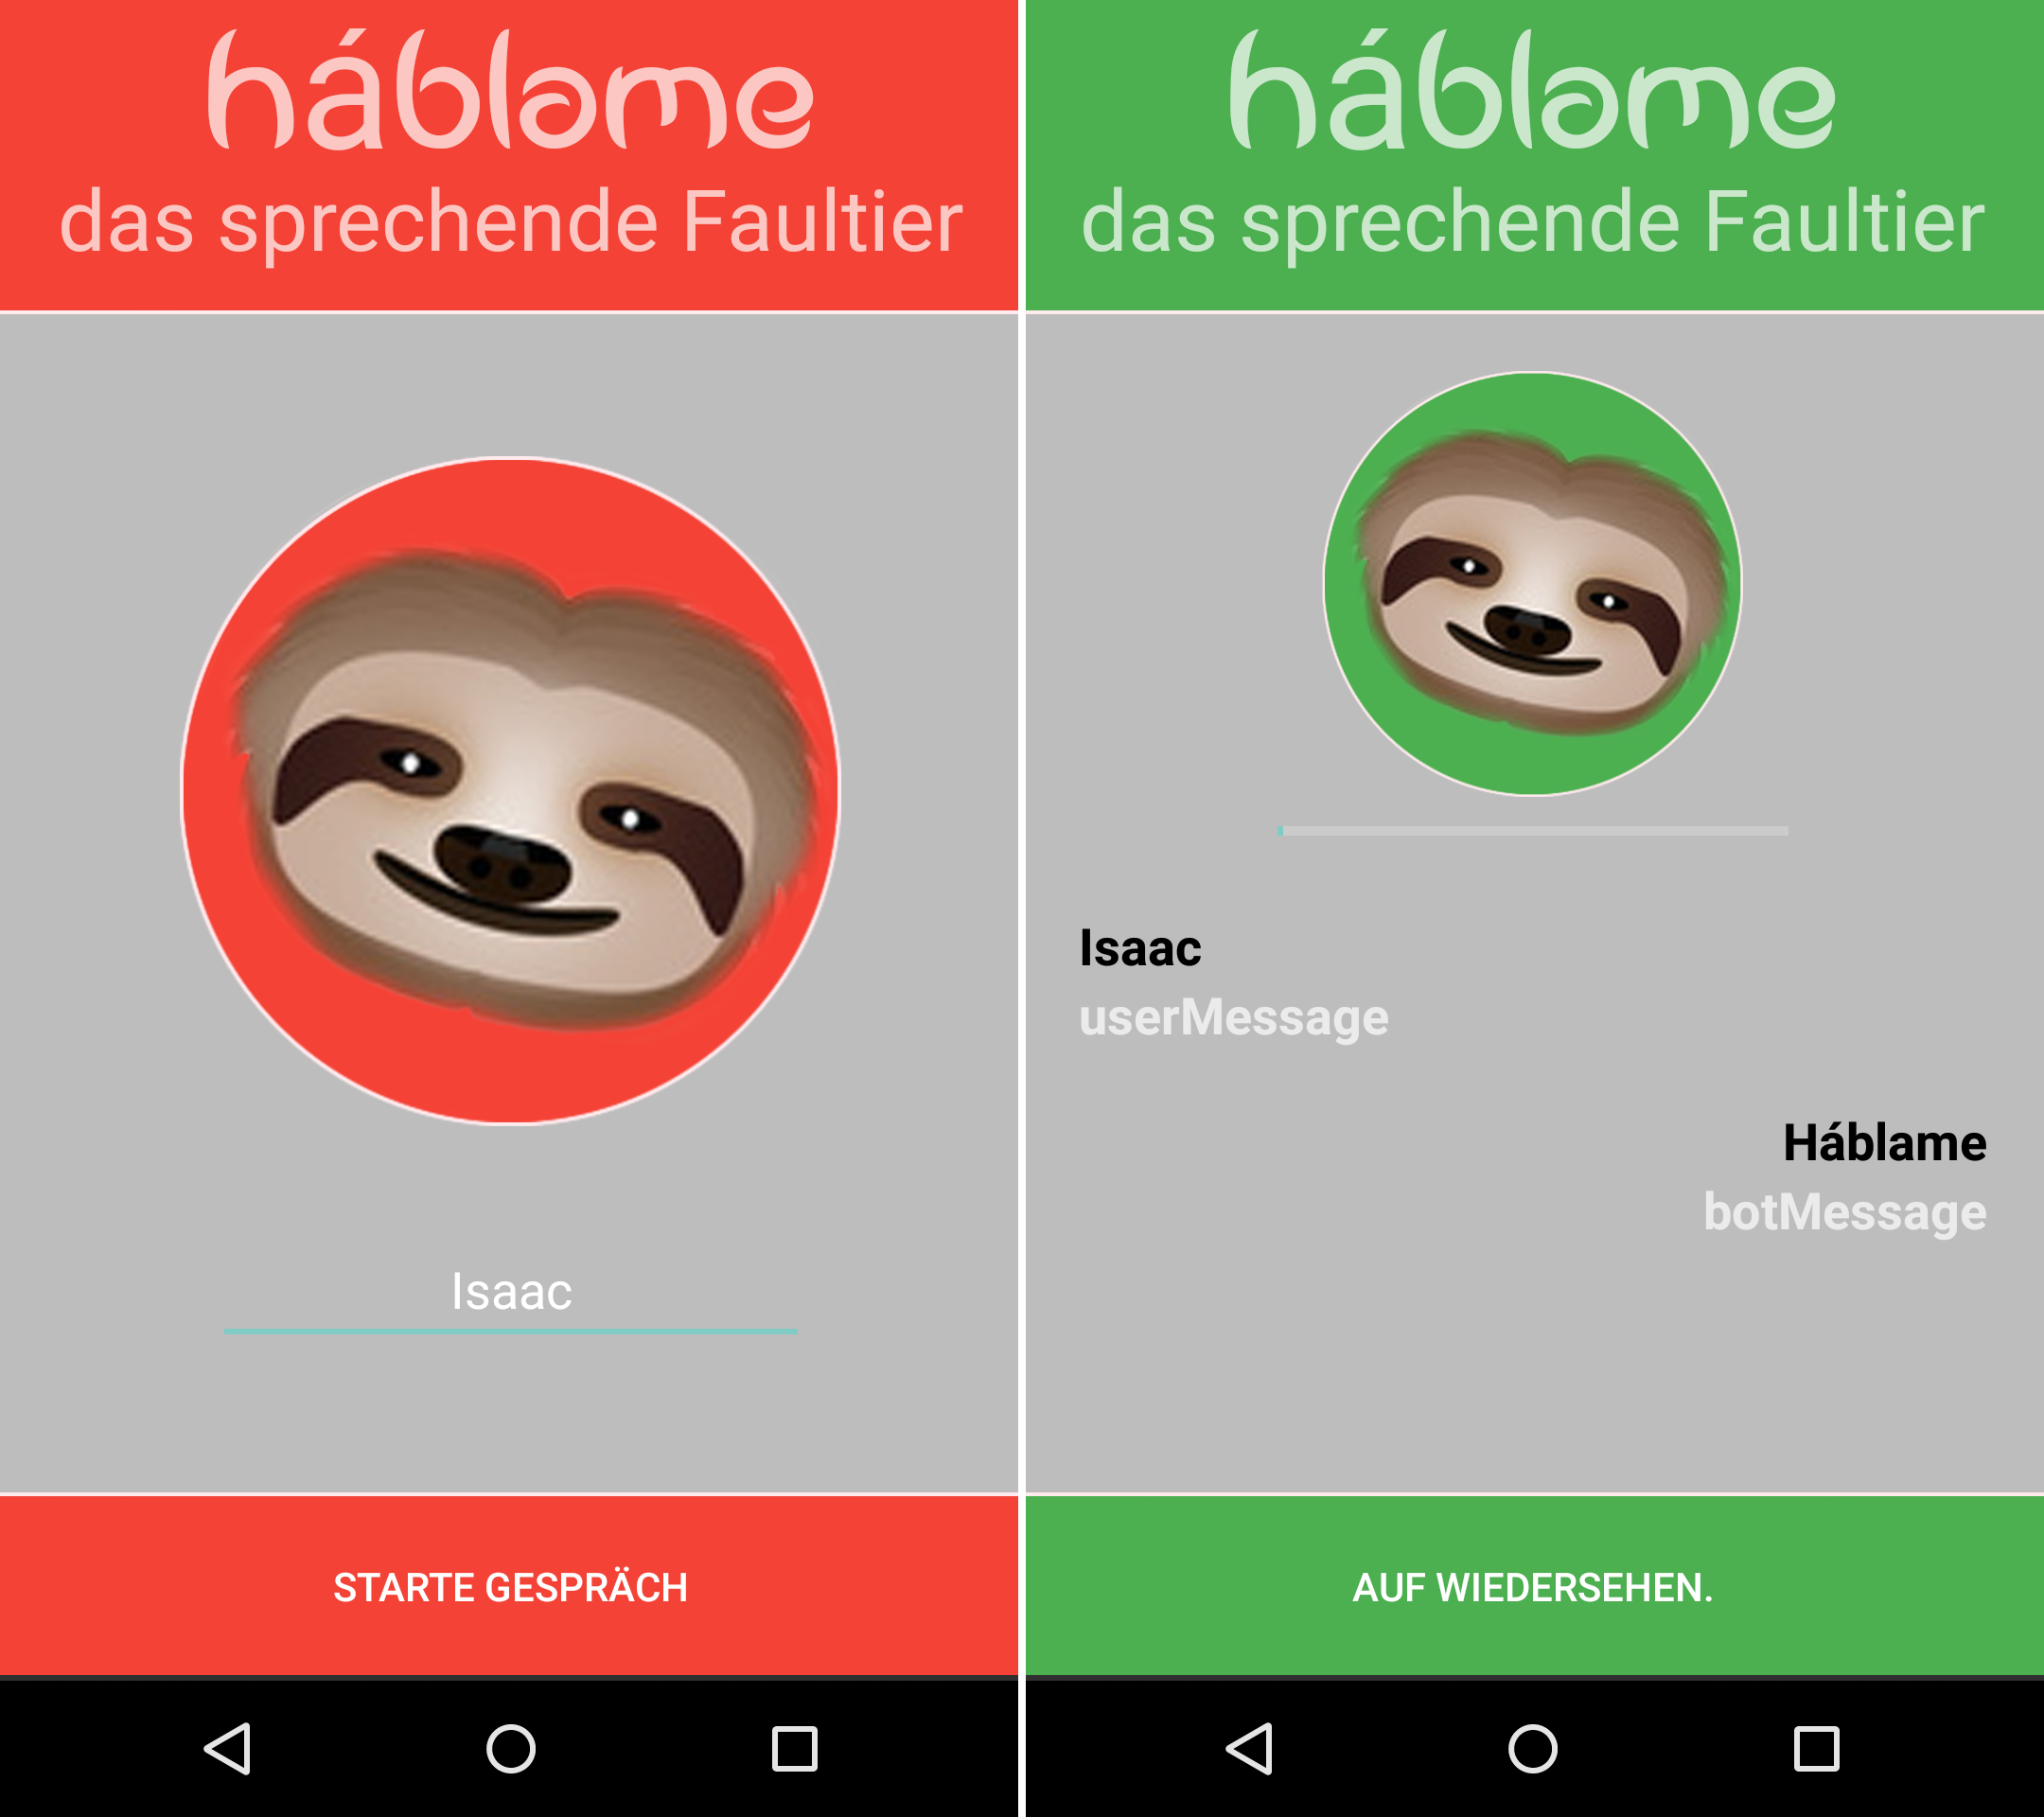
\includegraphics[width=1.0\linewidth]{dh/graphics/hablame-new.png}
		\caption{UI der neuen Android App}
		\label{fig:hablame-new}
	\end{figure}
	\newpage
	
	\section{Ausblick und Anregungen}
	\textsl{hier kommen die Dinge rein, welche noch zu machen sind:}
	\begin{itemize}\itemsep0pt
		\item{TLS Zertifikat für den Webserver und den Tomcatserver}
		\item{Mehr Extensions nutzen für externes Wissen (wie Wetter)}
		\item{Mehrbenutzerbetrieb (gehaltenes Wissen des Bots pro User)}
		\item{Pädagogenschnittstelle: Eigenständige Software, die die AIML-Syntax
		parst und Einträge bearbeiten kann}
		\item{Android Design Änderungen in der App}
	\end{itemize}
\end{document}
